
\begin{frame}

\begin{block}{
\begin{center}\Large CLASS\end{center}}
\begin{center}\small Cosmological Linear Anisotropy Solving System \end{center}
\end{block}

\scriptsize

\begin{center}
	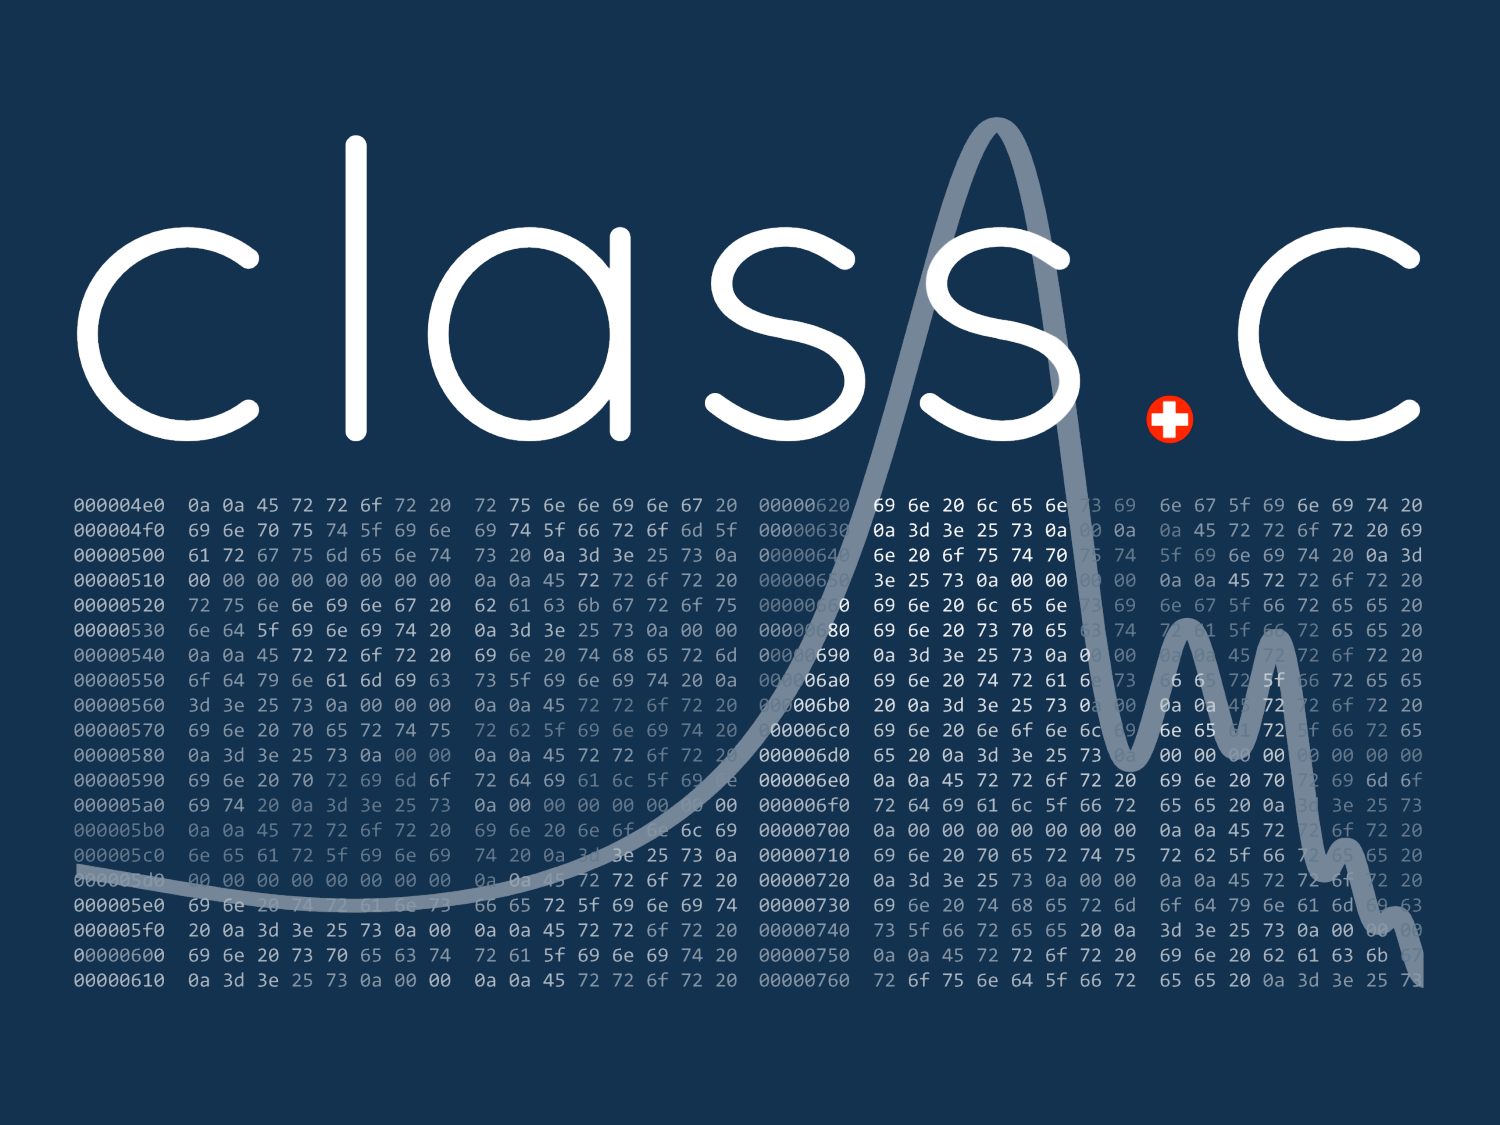
\includegraphics[width=5cm,angle=0]{Figures/Logo1b_blue.pdf}\\
	%\framebox{
	Markus Mosbech\\
	Institute for Theoretical Particle Physics, KIT\\
	\&\\
	Institute for Theoretical Particle Physics and Cosmology, RWTH\\
	\mbox{}\\
	\mbox{}\\
	\location, \ecolefromdate{}-\ecoletodate{} Oct 2025
	%}
	\vfill
	These slides available at \url{https://github.com/MarkMos/class_lecture}\\
	Visit \url{http://class-code.net/} for more info!
\end{center}

\end{frame}
